\documentclass{article}\usepackage[]{graphicx}\usepackage[]{xcolor}
% maxwidth is the original width if it is less than linewidth
% otherwise use linewidth (to make sure the graphics do not exceed the margin)
\makeatletter
\def\maxwidth{ %
  \ifdim\Gin@nat@width>\linewidth
    \linewidth
  \else
    \Gin@nat@width
  \fi
}
\makeatother

\definecolor{fgcolor}{rgb}{0.345, 0.345, 0.345}
\newcommand{\hlnum}[1]{\textcolor[rgb]{0.686,0.059,0.569}{#1}}%
\newcommand{\hlstr}[1]{\textcolor[rgb]{0.192,0.494,0.8}{#1}}%
\newcommand{\hlcom}[1]{\textcolor[rgb]{0.678,0.584,0.686}{\textit{#1}}}%
\newcommand{\hlopt}[1]{\textcolor[rgb]{0,0,0}{#1}}%
\newcommand{\hlstd}[1]{\textcolor[rgb]{0.345,0.345,0.345}{#1}}%
\newcommand{\hlkwa}[1]{\textcolor[rgb]{0.161,0.373,0.58}{\textbf{#1}}}%
\newcommand{\hlkwb}[1]{\textcolor[rgb]{0.69,0.353,0.396}{#1}}%
\newcommand{\hlkwc}[1]{\textcolor[rgb]{0.333,0.667,0.333}{#1}}%
\newcommand{\hlkwd}[1]{\textcolor[rgb]{0.737,0.353,0.396}{\textbf{#1}}}%
\let\hlipl\hlkwb

\usepackage{framed}
\makeatletter
\newenvironment{kframe}{%
 \def\at@end@of@kframe{}%
 \ifinner\ifhmode%
  \def\at@end@of@kframe{\end{minipage}}%
  \begin{minipage}{\columnwidth}%
 \fi\fi%
 \def\FrameCommand##1{\hskip\@totalleftmargin \hskip-\fboxsep
 \colorbox{shadecolor}{##1}\hskip-\fboxsep
     % There is no \\@totalrightmargin, so:
     \hskip-\linewidth \hskip-\@totalleftmargin \hskip\columnwidth}%
 \MakeFramed {\advance\hsize-\width
   \@totalleftmargin\z@ \linewidth\hsize
   \@setminipage}}%
 {\par\unskip\endMakeFramed%
 \at@end@of@kframe}
\makeatother

\definecolor{shadecolor}{rgb}{.97, .97, .97}
\definecolor{messagecolor}{rgb}{0, 0, 0}
\definecolor{warningcolor}{rgb}{1, 0, 1}
\definecolor{errorcolor}{rgb}{1, 0, 0}
\newenvironment{knitrout}{}{} % an empty environment to be redefined in TeX

\usepackage{alltt}
\usepackage[utf8]{inputenc}

%%% Load some LaTeX packages:
\usepackage[utf8]{inputenc}
\usepackage[nottoc,numbib]{tocbibind}      % for bibliography in the table of contents
\usepackage{hyperref}                      % link to website: \url{}.
\usepackage[hang,footnotesize,bf]{caption} % customized caption
\usepackage{amsmath}                       % for mathematical features 
\usepackage[left=2.5cm,top=3cm,bottom=3cm,right=2.5cm]{geometry}   % text margins
\usepackage{booktabs}                      % for booktabs in print(xtable)).
\usepackage{authblk}                       % for footnote style author/affiliation
\usepackage{float}
\usepackage{subfig}
\usepackage{bbm}              % for \mathbbm
\newcommand{\I}{\mathbbm{1}}  % shortcut for indicator function
\usepackage{enumitem}
\usepackage{dsfont}
\usepackage{cancel}

\usepackage{titling}
%\renewcommand\maketitlehooka{\null\mbox{}\vfill}
%\renewcommand\maketitlehookd{\vfill\null}

\usepackage{hyperref}
\hypersetup{
    colorlinks=true,
    linkcolor=blue,
    filecolor=magenta,      
    urlcolor=cyan,
    pdftitle={Overleaf Example},
    pdfpagemode=FullScreen,
    }

%%% Some LaTeX "macros":
\newcommand{\R}{\textsf{R}}
\newcommand{\Rpackage}[1]{\textsf{#1}}
\newcommand{\Robject}[1]{\texttt{#1}}

\newcommand{\hltexttt}[1]{\texttt{\hl{#1}}}







\IfFileExists{upquote.sty}{\usepackage{upquote}}{}
\begin{document}

\title{Data Analysis of DiaHelp user}
\author{Internet of things}
\maketitle
\section{Introduction}
For this data analysis we will have to interpret the results for the data we have, and since it is not real data, it may show incoherent results. Here we start at a point where we have a new measurement found on {\it measurement.json}.

\section{Reading the new measurement}
Since the measurement we get is received in json format, we use the library {\tt rjson} to import this data to the script. Then we transform this data to a data frame and select the wanted columns.
\begin{knitrout}\footnotesize
\definecolor{shadecolor}{rgb}{0.969, 0.969, 0.969}\color{fgcolor}\begin{kframe}
\begin{alltt}
\hlstd{> }\hlkwd{library}\hlstd{(rjson)}
\hlstd{> }\hlstd{js} \hlkwb{<-} \hlkwd{fromJSON}\hlstd{(}\hlkwc{file} \hlstd{=} \hlstr{"../measurement.json"}\hlstd{)}
\hlstd{> }\hlstd{df} \hlkwb{<-} \hlkwd{as.data.frame}\hlstd{(js)}
\hlstd{> }\hlstd{df} \hlkwb{<-} \hlstd{df[,}\hlkwd{c}\hlstd{(}\hlstr{"phone_number"}\hlstd{,} \hlstr{"age"}\hlstd{,} \hlstr{"gender"}\hlstd{,} \hlstr{"full_name"}\hlstd{,} \hlstr{"sensors.name"}
\hlstd{+ }      \hlstd{,}\hlstr{"sensors.data"}\hlstd{,} \hlstr{"sensors.unit_of_measurement"}
\hlstd{+ }      \hlstd{,}\hlstr{"sensors.name.1"}\hlstd{,} \hlstr{"sensors.data.1"}\hlstd{,} \hlstr{"sensors.unit_of_measurement.1"}
\hlstd{+ }      \hlstd{,}\hlstr{"sensors.name.2"}\hlstd{,} \hlstr{"sensors.data.2"}\hlstd{,} \hlstr{"sensors.unit_of_measurement.2"}
\hlstd{+ }      \hlstd{,}\hlstr{"sensors.name.3"}\hlstd{,} \hlstr{"sensors.data.3"}\hlstd{,} \hlstr{"sensors.unit_of_measurement.3"}\hlstd{)]}
\end{alltt}
\end{kframe}
\end{knitrout}

\section{Simulating data}
Medical data is sensitive and hard to find a good dataset on the Internet, that is the reason why we had to simulate our data, though, and the end of the day we have generated random data.
\\We needed an historic of the user that is why we have generated 1000 measurements for each sensor.
All the different data follows a normal distribution, and it is clearly seen when we plot an histogram of the variable of the measurement for each sensor.
\subsection*{Glucose levels simulation}
We have decided to generate random data following a normal distribution with mean of 120 and a standard deviation of 40. This numbers are an estimation done by ourselves after reading information on \url{https://www.healthline.com/health/diabetes/blood-sugar-level-chart#recommended-ranges}.
\begin{knitrout}\footnotesize
\definecolor{shadecolor}{rgb}{0.969, 0.969, 0.969}\color{fgcolor}\begin{kframe}
\begin{alltt}
\hlstd{> }\hlstd{sim_gc} \hlkwb{<-} \hlkwd{rnorm}\hlstd{(}\hlnum{1000}\hlstd{,} \hlkwc{mean} \hlstd{=} \hlnum{120}\hlstd{,} \hlkwc{sd} \hlstd{=} \hlnum{40}\hlstd{)}
\hlstd{> }\hlkwd{hist}\hlstd{(sim_gc,} \hlkwc{xlab} \hlstd{=} \hlstr{"Glucose levels"}\hlstd{,} \hlkwc{main} \hlstd{=} \hlstr{"Histogram of Glucose levels"}\hlstd{)}
\end{alltt}
\end{kframe}

{\centering 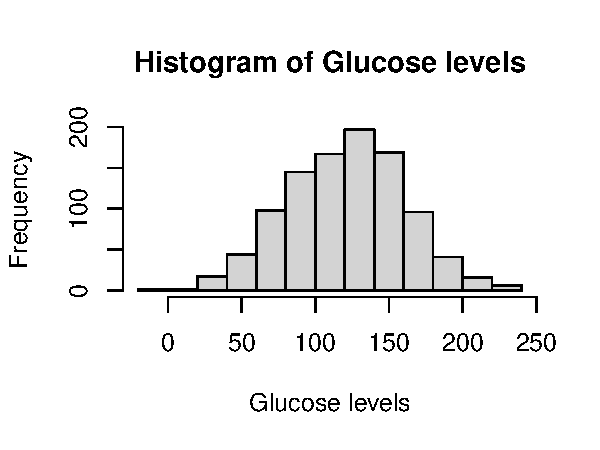
\includegraphics[width=\maxwidth]{figure/sim_gc-1} 

}


\end{knitrout}
\subsection*{Blood pressure simulation}
We have decided to generate random data following a normal distribution with mean of 110 and a standard deviation of 15. This numbers are an estimation done by ourselves after reading information on \url{https://www.emedicinehealth.com/what_is_a_normal_blood_pressure_range_by_age/article_em.htm}.
\begin{knitrout}\footnotesize
\definecolor{shadecolor}{rgb}{0.969, 0.969, 0.969}\color{fgcolor}\begin{kframe}
\begin{alltt}
\hlstd{> }\hlstd{sim_bp} \hlkwb{<-} \hlkwd{rnorm}\hlstd{(}\hlnum{1000}\hlstd{,} \hlkwc{mean} \hlstd{=} \hlnum{110}\hlstd{,} \hlkwc{sd} \hlstd{=} \hlnum{15}\hlstd{)}
\hlstd{> }\hlkwd{hist}\hlstd{(sim_bp,} \hlkwc{xlab} \hlstd{=} \hlstr{"Blood pressure"}\hlstd{,} \hlkwc{main} \hlstd{=} \hlstr{"Histogram of Blood pressure"}\hlstd{)}
\end{alltt}
\end{kframe}

{\centering 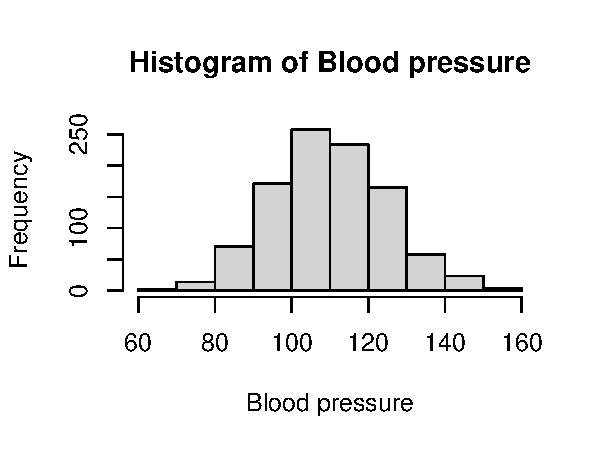
\includegraphics[width=\maxwidth]{figure/sim_bp-1} 

}


\end{knitrout}
\subsection*{Heart rate simulation}
We have decided to generate random data following a normal distribution with mean of 40 and a standard deviation of 10. This numbers are an estimation done by ourselves after reading information on \url{https://www.whoop.com/thelocker/normal-hrv-range-age-gender/}.
\begin{knitrout}\footnotesize
\definecolor{shadecolor}{rgb}{0.969, 0.969, 0.969}\color{fgcolor}\begin{kframe}
\begin{alltt}
\hlstd{> }\hlstd{sim_hr} \hlkwb{<-} \hlkwd{rnorm}\hlstd{(}\hlnum{1000}\hlstd{,} \hlkwc{mean} \hlstd{=} \hlnum{40}\hlstd{,} \hlkwc{sd} \hlstd{=} \hlnum{10}\hlstd{)}
\hlstd{> }\hlkwd{hist}\hlstd{(sim_hr,} \hlkwc{xlab} \hlstd{=} \hlstr{"Heart rate"}\hlstd{,} \hlkwc{main} \hlstd{=} \hlstr{"Histogram of Heart rate"}\hlstd{)}
\end{alltt}
\end{kframe}

{\centering 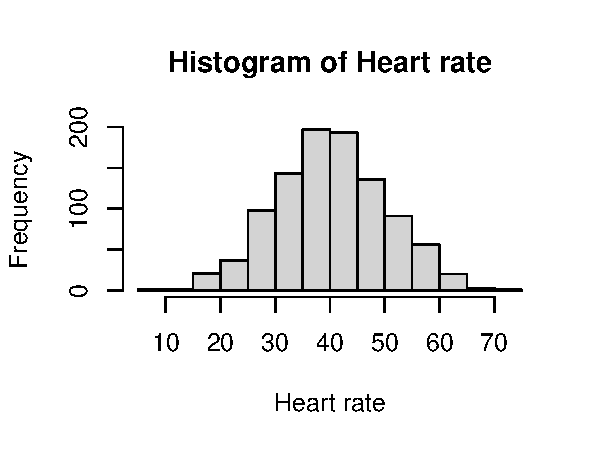
\includegraphics[width=\maxwidth]{figure/sim_hr-1} 

}


\end{knitrout}
\subsection*{Oxygen in blood simulation}
We have decided to generate random data following a normal distribution with mean of 96 and a standard deviation of 3. This numbers are an estimation done by ourselves after reading information on \url{https://www.emedicinehealth.com/what_is_a_good_oxygen_rate_by_age/article_em.htm}.
\begin{knitrout}\footnotesize
\definecolor{shadecolor}{rgb}{0.969, 0.969, 0.969}\color{fgcolor}\begin{kframe}
\begin{alltt}
\hlstd{> }\hlstd{sim_ob} \hlkwb{<-} \hlkwd{rnorm}\hlstd{(}\hlnum{1000}\hlstd{,} \hlkwc{mean} \hlstd{=} \hlnum{96}\hlstd{,} \hlkwc{sd} \hlstd{=} \hlnum{3}\hlstd{)}
\hlstd{> }\hlkwd{hist}\hlstd{(sim_ob,} \hlkwc{xlab} \hlstd{=} \hlstr{"Oxygen in blood"}\hlstd{,} \hlkwc{main} \hlstd{=} \hlstr{"Histogram of Oxygen in blood"}\hlstd{)}
\end{alltt}
\end{kframe}

{\centering 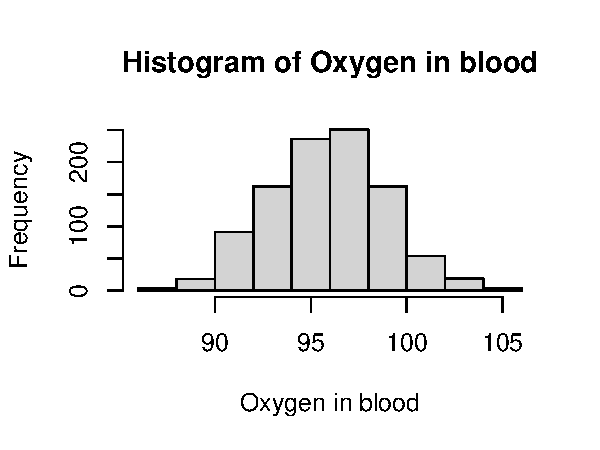
\includegraphics[width=\maxwidth]{figure/sim_ob-1} 

}


\end{knitrout}
\subsection*{Merging all new data}
Now we want to have all this data together as we could have it in our database, so merge all the data in a data frame. This is the replacement of the historic of the user that we don't have.
\begin{knitrout}\footnotesize
\definecolor{shadecolor}{rgb}{0.969, 0.969, 0.969}\color{fgcolor}\begin{kframe}
\begin{alltt}
\hlstd{> }\hlstd{historic} \hlkwb{<-} \hlkwd{data.frame}\hlstd{(}
\hlstd{+ }  \hlstr{"glucose levels (mg/dl)"} \hlstd{= sim_gc}
\hlstd{+ }  \hlstd{,}\hlstr{"blood pressure (mm/Hg)"} \hlstd{= sim_bp}
\hlstd{+ }  \hlstd{,}\hlstr{"heart rate (HRV)"} \hlstd{= sim_hr}
\hlstd{+ }  \hlstd{,}\hlstr{"oxygen levels (HRV)"} \hlstd{= sim_ob}
\hlstd{+ }  \hlstd{,}\hlkwc{check.names}\hlstd{=}\hlnum{FALSE}
\hlstd{+ }\hlstd{)}
\end{alltt}
\end{kframe}
\end{knitrout}
\section{Correlation study between variables}
Our project is focused on diabetic people, that is why we studied the glucose levels against the other variables to see if there is any correlation between them. This has been done performing a Pearson Hypothesis Test, where the null hypothesis $H_0$ is "there is not correlation", and the alternative hypothesis $H_1$, "there is correlation" between the variables of the measurements.
\subsection*{Glucose levels vs. Blood pressure}
First of all a plot, with glucose levels on x-axis and blood pressure on y-axis.
\begin{knitrout}\footnotesize
\definecolor{shadecolor}{rgb}{0.969, 0.969, 0.969}\color{fgcolor}\begin{kframe}
\begin{alltt}
\hlstd{> }\hlkwd{plot}\hlstd{(historic}\hlopt{$}\hlstd{`glucose levels (mg/dl)`, historic}\hlopt{$}\hlstd{`blood pressure (mm/Hg)`,}
\hlstd{+ }     \hlkwc{xlab} \hlstd{=} \hlstr{"Glucose levels"}\hlstd{,} \hlkwc{ylab} \hlstd{=} \hlstr{"Blood pressure"}\hlstd{,}
\hlstd{+ }     \hlkwc{main} \hlstd{=} \hlstr{"Glcuose levels vs Blood pressure"}\hlstd{)}
\end{alltt}
\end{kframe}

{\centering 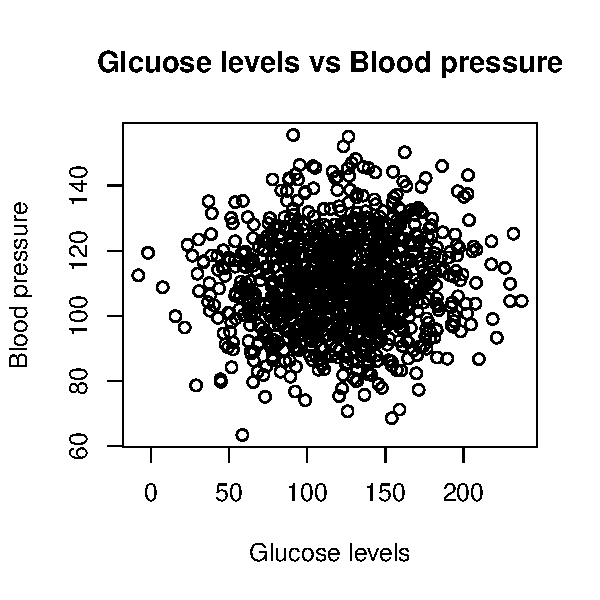
\includegraphics[width=\maxwidth]{figure/plt_bp-1} 

}


\end{knitrout}
\noindent From the plot we can already expect there won't be any correlation. With the correlation test we can confirm that.
\begin{knitrout}\footnotesize
\definecolor{shadecolor}{rgb}{0.969, 0.969, 0.969}\color{fgcolor}\begin{kframe}
\begin{alltt}
\hlstd{> }\hlstd{test_gc} \hlkwb{<-} \hlkwd{cor.test}\hlstd{(historic}\hlopt{$}\hlstd{`glucose levels (mg/dl)`, historic}\hlopt{$}\hlstd{`blood pressure (mm/Hg)`)}
\hlstd{> }\hlkwd{print}\hlstd{(test_gc)}
\end{alltt}
\begin{verbatim}
## 
## 	Pearson's product-moment correlation
## 
## data:  historic$`glucose levels (mg/dl)` and historic$`blood pressure (mm/Hg)`
## t = 1.8026, df = 998, p-value = 0.07176
## alternative hypothesis: true correlation is not equal to 0
## 95 percent confidence interval:
##  -0.005043824  0.118541517
## sample estimates:
##        cor 
## 0.05696707
\end{verbatim}
\end{kframe}
\end{knitrout}
\noindent The correlation coefficient between the two vectors turns out to be 0.0569671. A positive correlation would be near 1, a negative one near -1, and no correlation near 0. The p-value is 0.0717555, higher than 0.05, so we decide to believe that we cannot fail to reject the null hypothesis, hence there is no correlation between the glucose levels and the blood pressure.
\subsection*{Glucose levels vs. Heart rate}
First of all a plot, with glucose levels on x-axis and heart rate on y-axis.
\begin{knitrout}\footnotesize
\definecolor{shadecolor}{rgb}{0.969, 0.969, 0.969}\color{fgcolor}\begin{kframe}
\begin{alltt}
\hlstd{> }\hlkwd{plot}\hlstd{(historic}\hlopt{$}\hlstd{`glucose levels (mg/dl)`, historic}\hlopt{$}\hlstd{`heart rate (HRV)`,}
\hlstd{+ }     \hlkwc{xlab} \hlstd{=} \hlstr{"Glucose levels"}\hlstd{,} \hlkwc{ylab} \hlstd{=} \hlstr{"Heart rate"}\hlstd{,}
\hlstd{+ }     \hlkwc{main} \hlstd{=} \hlstr{"Glcuose levels vs Heart rate"}\hlstd{)}
\end{alltt}
\end{kframe}

{\centering 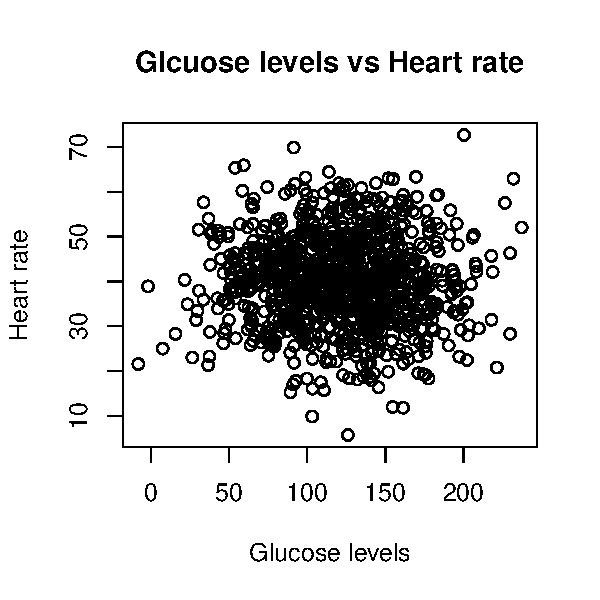
\includegraphics[width=\maxwidth]{figure/plt_hr-1} 

}


\end{knitrout}
\noindent From the plot we can already expect there won't be any correlation. With the correlation test we can confirm that.
\begin{knitrout}\footnotesize
\definecolor{shadecolor}{rgb}{0.969, 0.969, 0.969}\color{fgcolor}\begin{kframe}
\begin{alltt}
\hlstd{> }\hlstd{test_hr} \hlkwb{<-} \hlkwd{cor.test}\hlstd{(historic}\hlopt{$}\hlstd{`glucose levels (mg/dl)`, historic}\hlopt{$}\hlstd{`heart rate (HRV)`)}
\hlstd{> }\hlkwd{print}\hlstd{(test_hr)}
\end{alltt}
\begin{verbatim}
## 
## 	Pearson's product-moment correlation
## 
## data:  historic$`glucose levels (mg/dl)` and historic$`heart rate (HRV)`
## t = -0.40618, df = 998, p-value = 0.6847
## alternative hypothesis: true correlation is not equal to 0
## 95 percent confidence interval:
##  -0.07478986  0.04917589
## sample estimates:
##         cor 
## -0.01285638
\end{verbatim}
\end{kframe}
\end{knitrout}
\noindent The correlation coefficient between the two vectors turns out to be -0.0128564. A positive correlation would be near 1, a negative one near -1, and no correlation near 0. The p-value is 0.6846964, higher than 0.05, so we decide to believe that we cannot fail to reject the null hypothesis, hence there is no correlation between the glucose levels and the blood pressure.
\subsection*{Glucose levels vs. Oxygen in blood}
First of all a plot, with glucose levels on x-axis and oxygen levels on y-axis.
\begin{knitrout}\footnotesize
\definecolor{shadecolor}{rgb}{0.969, 0.969, 0.969}\color{fgcolor}\begin{kframe}
\begin{alltt}
\hlstd{> }\hlkwd{plot}\hlstd{(historic}\hlopt{$}\hlstd{`glucose levels (mg/dl)`, historic}\hlopt{$}\hlstd{`oxygen levels (HRV)`,}
\hlstd{+ }     \hlkwc{xlab} \hlstd{=} \hlstr{"Glucose levels"}\hlstd{,} \hlkwc{ylab} \hlstd{=} \hlstr{"Oxygen in blood"}\hlstd{,}
\hlstd{+ }     \hlkwc{main} \hlstd{=} \hlstr{"Glcuose levels vs Oxygen in blood"}\hlstd{)}
\end{alltt}
\end{kframe}

{\centering 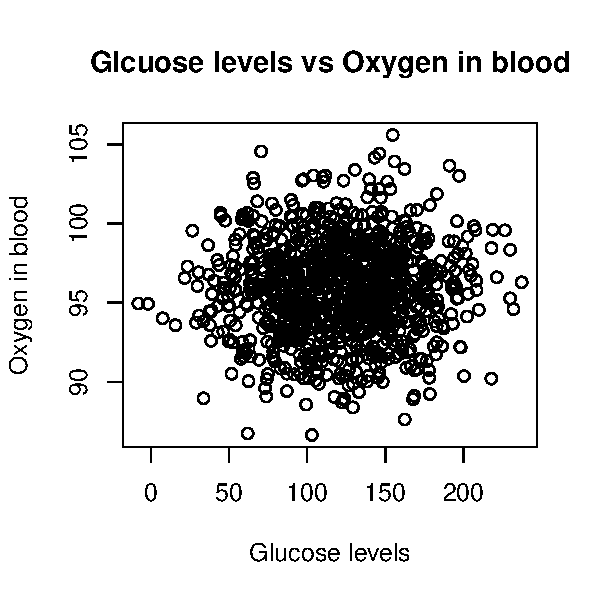
\includegraphics[width=\maxwidth]{figure/plt_ol-1} 

}


\end{knitrout}
\noindent From the plot we can already expect there won't be any correlation. With the correlation test we can confirm that.
\begin{knitrout}\footnotesize
\definecolor{shadecolor}{rgb}{0.969, 0.969, 0.969}\color{fgcolor}\begin{kframe}
\begin{alltt}
\hlstd{> }\hlstd{test_ol} \hlkwb{<-} \hlkwd{cor.test}\hlstd{(historic}\hlopt{$}\hlstd{`glucose levels (mg/dl)`, historic}\hlopt{$}\hlstd{`oxygen levels (HRV)`)}
\hlstd{> }\hlkwd{print}\hlstd{(test_ol)}
\end{alltt}
\begin{verbatim}
## 
## 	Pearson's product-moment correlation
## 
## data:  historic$`glucose levels (mg/dl)` and historic$`oxygen levels (HRV)`
## t = 1.2135, df = 998, p-value = 0.2252
## alternative hypothesis: true correlation is not equal to 0
## 95 percent confidence interval:
##  -0.0236639  0.1001403
## sample estimates:
##       cor 
## 0.0383855
\end{verbatim}
\end{kframe}
\end{knitrout}
\noindent The correlation coefficient between the two vectors turns out to be 0.0383855. A positive correlation would be near 1, a negative one near -1, and no correlation near 0. The p-value is 0.2252121, higher than 0.05, so we decide to believe that we cannot fail to reject the null hypothesis, hence there is no correlation between the glucose levels and the blood pressure.
\section{Abnormal measurements}
For the new measurement we have taken from the user we now want to check if the values are normal for they history because in case they are not they could be in a potential risk of an emergency situation and they could need help. So for this section we are going to construct $99\%$ confidence intervals and raise a message in case the new value is out of the bounds of the interval.
\\\\
First we need to compute the {\it t-score} for a $99\%$ confidence.
\begin{knitrout}\footnotesize
\definecolor{shadecolor}{rgb}{0.969, 0.969, 0.969}\color{fgcolor}\begin{kframe}
\begin{alltt}
\hlstd{> }\hlcom{# length of the historic}
\hlstd{> }\hlstd{n} \hlkwb{<-} \hlkwd{length}\hlstd{(historic}\hlopt{$}\hlstd{`glucose levels (mg/dl)`)}
\hlstd{> }
\hlstd{> }\hlcom{# calculate t-value for 99% confidence}
\hlstd{> }\hlstd{alpha} \hlkwb{=} \hlnum{0.01}
\hlstd{> }\hlstd{degrees_of_freedom} \hlkwb{=} \hlstd{n} \hlopt{-} \hlnum{1}
\hlstd{> }\hlstd{t_score} \hlkwb{=} \hlkwd{qt}\hlstd{(}\hlkwc{p}\hlstd{=alpha}\hlopt{/}\hlnum{2}\hlstd{,} \hlkwc{df}\hlstd{=degrees_of_freedom,}\hlkwc{lower.tail}\hlstd{=F)}
\end{alltt}
\end{kframe}
\end{knitrout}
\subsection*{Glucose levels}
Having the {\it t-score} we now can construct the interval. For the glucose levels:
\begin{knitrout}\footnotesize
\definecolor{shadecolor}{rgb}{0.969, 0.969, 0.969}\color{fgcolor}\begin{kframe}
\begin{alltt}
\hlstd{> }\hlcom{# confidence interval for glucose levels}
\hlstd{> }\hlstd{X} \hlkwb{<-} \hlkwd{mean}\hlstd{(historic}\hlopt{$}\hlstd{`glucose levels (mg/dl)`)}
\hlstd{> }\hlstd{sd} \hlkwb{<-} \hlkwd{sd}\hlstd{(historic}\hlopt{$}\hlstd{`glucose levels (mg/dl)`)}
\hlstd{> }\hlstd{std_error} \hlkwb{<-} \hlstd{sd} \hlopt{/} \hlkwd{sqrt}\hlstd{(n)}
\hlstd{> }\hlstd{margin_error} \hlkwb{<-} \hlstd{t_score} \hlopt{*} \hlstd{std_error}
\hlstd{> }\hlstd{up_bound_gc} \hlkwb{<-} \hlstd{X} \hlopt{+} \hlstd{margin_error}
\hlstd{> }\hlstd{low_bound_gc} \hlkwb{<-} \hlstd{X} \hlopt{-} \hlstd{margin_error}
\end{alltt}
\end{kframe}
\end{knitrout}
\noindent The lower bound of the interval is 117.6988738, the mean is 120.9454389 and the upper bound 124.192004. And with the first data frame we built for the new measurement we can check if the new input value is in the normal values of the user.
\begin{knitrout}\footnotesize
\definecolor{shadecolor}{rgb}{0.969, 0.969, 0.969}\color{fgcolor}\begin{kframe}
\begin{alltt}
\hlstd{> }\hlkwa{if} \hlstd{(df}\hlopt{$}\hlstd{sensors.data} \hlopt{<} \hlstd{low_bound_gc} \hlopt{||} \hlstd{df}\hlopt{$}\hlstd{sensors.data} \hlopt{>} \hlstd{up_bound_gc)}
\hlstd{+ }  \hlkwd{print}\hlstd{(}\hlstr{"You should check your glucose levels!"}\hlstd{)}
\end{alltt}
\end{kframe}
\end{knitrout}
\noindent The new measurement is 120 mg/dl, since it inside the interval then there is nothing to alert.
\subsection*{Blood pressure}
For the blood pressure:
\begin{knitrout}\footnotesize
\definecolor{shadecolor}{rgb}{0.969, 0.969, 0.969}\color{fgcolor}\begin{kframe}
\begin{alltt}
\hlstd{> }\hlcom{# confidence interval for blood pressure}
\hlstd{> }\hlstd{X} \hlkwb{<-} \hlkwd{mean}\hlstd{(historic}\hlopt{$}\hlstd{`blood pressure (mm/Hg)`)}
\hlstd{> }\hlstd{sd} \hlkwb{<-} \hlkwd{sd}\hlstd{(historic}\hlopt{$}\hlstd{`blood pressure (mm/Hg)`)}
\hlstd{> }\hlstd{std_error} \hlkwb{<-} \hlstd{sd} \hlopt{/} \hlkwd{sqrt}\hlstd{(n)}
\hlstd{> }\hlstd{margin_error} \hlkwb{<-} \hlstd{t_score} \hlopt{*} \hlstd{std_error}
\hlstd{> }\hlstd{up_bound_bp} \hlkwb{<-} \hlstd{X} \hlopt{+} \hlstd{margin_error}
\hlstd{> }\hlstd{low_bound_bp} \hlkwb{<-} \hlstd{X} \hlopt{-} \hlstd{margin_error}
\end{alltt}
\end{kframe}
\end{knitrout}
\noindent The lower bound of the interval is 108.6629725, the mean is 109.8707757 and the upper bound 111.0785788. And with the first data frame we built for the new measurement we can check if the new input value is in the normal values of the user.
\begin{knitrout}\footnotesize
\definecolor{shadecolor}{rgb}{0.969, 0.969, 0.969}\color{fgcolor}\begin{kframe}
\begin{alltt}
\hlstd{> }\hlkwa{if} \hlstd{(df}\hlopt{$}\hlstd{sensors.data.1} \hlopt{<} \hlstd{low_bound_bp} \hlopt{||} \hlstd{df}\hlopt{$}\hlstd{sensors.data.1} \hlopt{>} \hlstd{up_bound_bp)}
\hlstd{+ }  \hlkwd{print}\hlstd{(}\hlstr{"You should check your blood pressure!"}\hlstd{)}
\end{alltt}
\begin{verbatim}
## [1] "You should check your blood pressure!"
\end{verbatim}
\end{kframe}
\end{knitrout}
\noindent The new measurement is 105 mm/Hg. In this situation the value is lower than the norm, so we notify the user to check his blood pressure.
\subsection*{Heart rate}
For the heart rate:
\begin{knitrout}\footnotesize
\definecolor{shadecolor}{rgb}{0.969, 0.969, 0.969}\color{fgcolor}\begin{kframe}
\begin{alltt}
\hlstd{> }\hlcom{# confidence interval for heart rate}
\hlstd{> }\hlstd{X} \hlkwb{<-} \hlkwd{mean}\hlstd{(historic}\hlopt{$}\hlstd{`heart rate (HRV)`)}
\hlstd{> }\hlstd{sd} \hlkwb{<-} \hlkwd{sd}\hlstd{(historic}\hlopt{$}\hlstd{`heart rate (HRV)`)}
\hlstd{> }\hlstd{std_error} \hlkwb{<-} \hlstd{sd} \hlopt{/} \hlkwd{sqrt}\hlstd{(n)}
\hlstd{> }\hlstd{margin_error} \hlkwb{<-} \hlstd{t_score} \hlopt{*} \hlstd{std_error}
\hlstd{> }\hlstd{up_bound_hr} \hlkwb{<-} \hlstd{X} \hlopt{+} \hlstd{margin_error}
\hlstd{> }\hlstd{low_bound_hr} \hlkwb{<-} \hlstd{X} \hlopt{-} \hlstd{margin_error}
\end{alltt}
\end{kframe}
\end{knitrout}
\noindent The lower bound of the interval is 39.3102688, the mean is 40.1295305 and the upper bound 40.9487923. And with the first data frame we built for the new measurement we can check if the new input value is in the normal values of the user.
\begin{knitrout}\footnotesize
\definecolor{shadecolor}{rgb}{0.969, 0.969, 0.969}\color{fgcolor}\begin{kframe}
\begin{alltt}
\hlstd{> }\hlkwa{if} \hlstd{(df}\hlopt{$}\hlstd{sensors.data.2} \hlopt{<} \hlstd{low_bound_hr} \hlopt{||} \hlstd{df}\hlopt{$}\hlstd{sensors.data.2} \hlopt{>} \hlstd{up_bound_hr)}
\hlstd{+ }  \hlkwd{print}\hlstd{(}\hlstr{"You should check your heart rate!"}\hlstd{)}
\end{alltt}
\end{kframe}
\end{knitrout}
\noindent The new measurement is 40 HRV, since it inside the interval then there is nothing to alert.
\subsection*{Oxygen in blood}
For the oxygen in blood:
\begin{knitrout}\footnotesize
\definecolor{shadecolor}{rgb}{0.969, 0.969, 0.969}\color{fgcolor}\begin{kframe}
\begin{alltt}
\hlstd{> }\hlcom{# confidence interval for oxygen levels}
\hlstd{> }\hlstd{X} \hlkwb{<-} \hlkwd{mean}\hlstd{(historic}\hlopt{$}\hlstd{`oxygen levels (HRV)`)}
\hlstd{> }\hlstd{sd} \hlkwb{<-} \hlkwd{sd}\hlstd{(historic}\hlopt{$}\hlstd{`oxygen levels (HRV)`)}
\hlstd{> }\hlstd{std_error} \hlkwb{<-} \hlstd{sd} \hlopt{/} \hlkwd{sqrt}\hlstd{(n)}
\hlstd{> }\hlstd{margin_error} \hlkwb{<-} \hlstd{t_score} \hlopt{*} \hlstd{std_error}
\hlstd{> }\hlstd{up_bound_ol} \hlkwb{<-} \hlstd{X} \hlopt{+} \hlstd{margin_error}
\hlstd{> }\hlstd{low_bound_ol} \hlkwb{<-} \hlstd{X} \hlopt{-} \hlstd{margin_error}
\end{alltt}
\end{kframe}
\end{knitrout}
\noindent The lower bound of the interval is 95.5900838, the mean is 95.8344372 and the upper bound 96.0787907. And with the first data frame we built for the new measurement we can check if the new input value is in the normal values of the user.
\begin{knitrout}\footnotesize
\definecolor{shadecolor}{rgb}{0.969, 0.969, 0.969}\color{fgcolor}\begin{kframe}
\begin{alltt}
\hlstd{> }\hlkwa{if} \hlstd{(df}\hlopt{$}\hlstd{sensors.data.3} \hlopt{<} \hlstd{low_bound_ol} \hlopt{||} \hlstd{df}\hlopt{$}\hlstd{sensors.data.3} \hlopt{>} \hlstd{up_bound_ol)}
\hlstd{+ }  \hlkwd{print}\hlstd{(}\hlstr{"You should check your oxygen levels!"}\hlstd{)}
\end{alltt}
\end{kframe}
\end{knitrout}
\noindent The new measurement is 96 HRV, since it inside the interval then there is nothing to alert.
\\\\
\section{Improve our data}
This new measurement can be used in the future to prevent unwanted situation, that is why we add it to the historic of the user.
\begin{knitrout}\footnotesize
\definecolor{shadecolor}{rgb}{0.969, 0.969, 0.969}\color{fgcolor}\begin{kframe}
\begin{alltt}
\hlstd{> }\hlstd{new_measurement} \hlkwb{<-} \hlkwd{c}\hlstd{(df}\hlopt{$}\hlstd{sensors.data, df}\hlopt{$}\hlstd{sensors.data.1, df}\hlopt{$}\hlstd{sensors.data.2, df}\hlopt{$}\hlstd{sensors.data.3)}
\hlstd{> }\hlstd{historic} \hlkwb{<-} \hlkwd{rbind}\hlstd{(historic, new_measurement)}
\end{alltt}
\end{kframe}
\end{knitrout}
\section{Results}
All the results shown in this analysis are the result of the randomly generated data with Gaussian distributions. That is why they don't reflect reality and we do not take responsibility for any misuse or misinterpretation of these results.
\\Since the data has been generated using a normal distribution, and independently one from another variable, it makes sense they are not correlated at all, however, we would probably see some if the data was from a real user. Another problem arises with the confidence intervals, which they are quite narrow due to how the data has been accuired.
\end{document}
